\section{Wed, Sep 12, 2018}

\begin{figure}[h!]
  \centering
  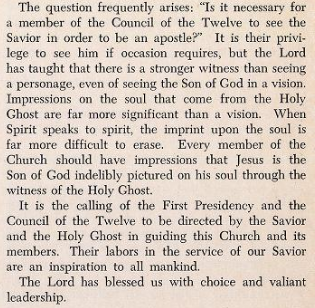
\includegraphics[width=.5\linewidth]{2018/images/apostle.png}
  \caption{Apostles Don't Need To See Christ}
  \label{fig:apostle}
\end{figure}

That quote is from the Improvement Era, Nov 1966, Page 979.

There's an interesting quote if you ask me. They're called as special witnesses of
Christ, but that appears to be in name only these days. In the old world, and in the
americas when Christ visited they were actual witnesses of Christ. For they saw and
talked and walked with Him. Nowadays? Not so much.

Makes one pause and wonder at times. If the church is actually being led by Jesus
Christ himself or just fuzzy warm thoughts and impressions that come to their mind?
They claim it to be revelation, but what exactly is revelation? I mean we have the
passage in the D\&C about it.

\begin{displayquote}
Yea, behold, I will tell you in your mind and in your heart, by the Holy Ghost, 
which shall come upon you and which shall dwell in your heart.

Now, behold, this is the spirit of revelation; behold, this is the spirit by which 
Moses brought the children of Israel through the Red Sea on dry ground.\footnote{
D\&C 8:2-3
}
\end{displayquote}

So, the Holy Ghost speaks to you through your mind and your heart. That's an
interesting thought process. The mind and heart are often at odds with each other,
well from personal experience. So when they are in harmony it is of God and they are
helping to channel revelation to you? Interesting thought for sure.